% Appendix C

\chapter{Statistical Tests} % Main appendix title

\label{AppendixC} % For referencing this appendix elsewhere, use \ref{AppendixA}

\lhead{Appendix C. \emph{Statistical Tests}} % This is for the header on each page - perhaps a shortened title

To substantiate our claim that stop word frequency varies according to header section, we computed the frequency of stops words in  abstract, author list, and title sections for 20 HEP papers (\texttt{anova\_data.py}). Plotting these frequencies (Figure \ref{fig:means}) showed a drastic difference

\begin{figure}[!ht]
\center
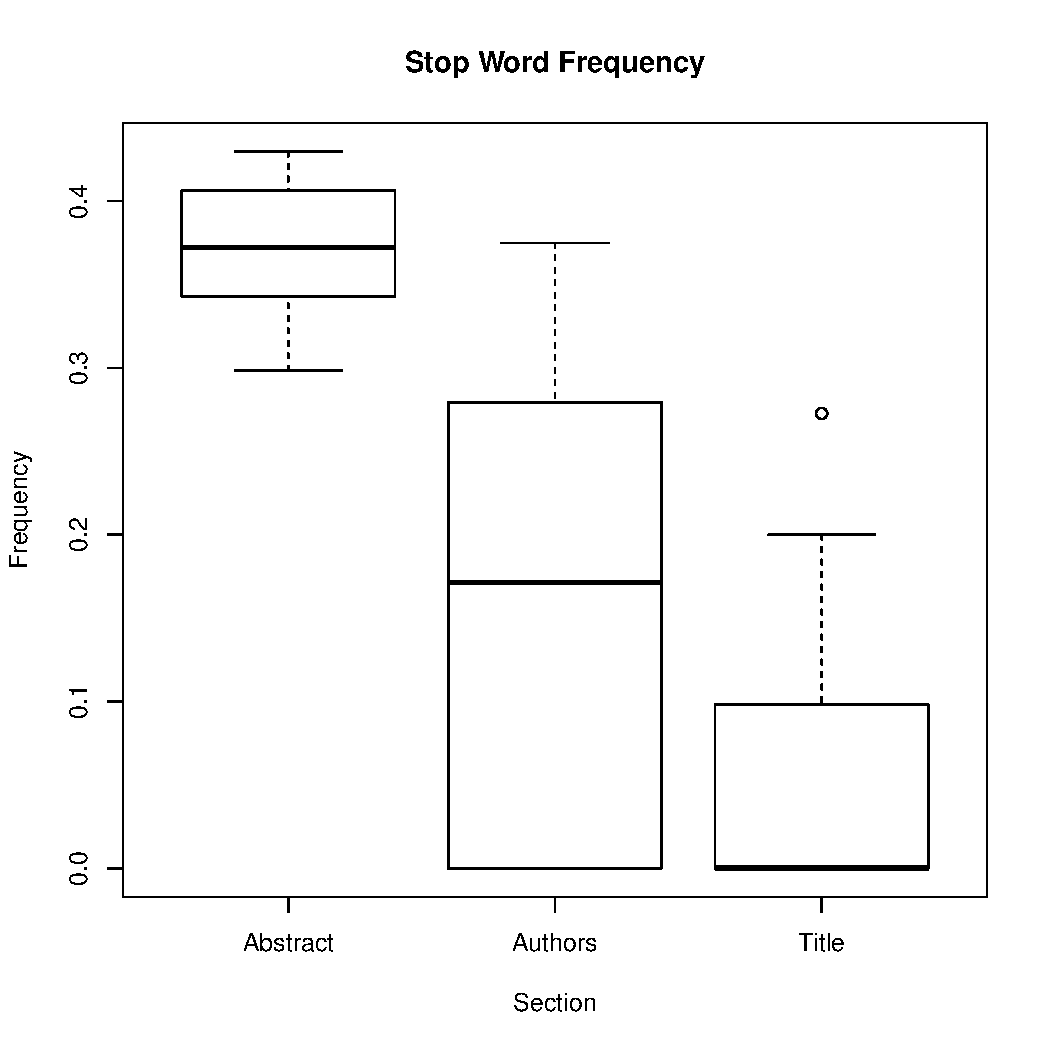
\includegraphics[width=4.5in]{Figures/means.pdf}
\caption{Box plots of stop word frequency according to header section.}
\label{fig:means}
\end{figure}

To confirm the significance of this result, we first performed an ANOVA (Figure \ref{fig:anova}) on the frequency data. The test reported a p-value of ($< 0.01$), permitting us to reject the null hypothesis that the means are equal ($\text{H}_0: \mu_1 = \mu_2 = \dots = \mu_k$), thereby confirming the statistical significance of the varying means. We further performed pairwise t tests (Figure \ref{fig:ttest}) to show the significance of the result for each class, with each p-value of ($< 0.01$).

\begin{figure}
\centering
\begin{BVerbatim}
            Df Sum Sq Mean Sq F value  Pr(>F)
Section      2 1.0685  0.5342   57.28 2.3e-14 ***
Residuals   57 0.5317  0.0093                    
---
Signif. codes:  0 ‘***’ 0.001 ‘**’ 0.01 ‘*’ 0.05 ‘.’ 0.1 ‘ ’ 1
\end{BVerbatim}
\caption{Excerpt of capitalisation features templates or \emph{macros}.}
\label{fig:anova}
\end{figure}

\begin{figure}
\centering
\begin{BVerbatim}
	Pairwise comparisons using t tests with pooled SD

data:  stops and sections

        Abstract Authors
Authors 1.5e-08  -      
Title   1.6e-14  0.0016

P value adjustment method: bonferroni
\end{BVerbatim}
\caption{Excerpt of capitalisation features templates or \emph{macros}.}
\label{fig:ttest}
\end{figure}
